\documentclass[10pt,a4paper]{report}

\usepackage{color}
\usepackage{graphicx}
\usepackage{wrapfig}
\usepackage[utf8x]{inputenc}
\usepackage{amssymb}
\usepackage{amsmath}
\usepackage{MnSymbol}
\usepackage[electronic]{ifsym}
\usepackage{listings}

\lstset{ %
%%% deletecomment=[l]--!,
language=VHDL,
%basicstyle=\footnotesize,
%numbers=left,
%numberstyle=\footnotesize,
%stepnumber=2,
numbersep=5pt,
%backgroundcolor=\color{white},
showspaces=false,
showstringspaces=false,
showtabs=false,
frame=single,
%tabsize=2,
captionpos=b,
breaklines=true,
breakatwhitespace=false,
title=\lstcaption,
%commentstyle=\color{blue},
}

\author{Ilya Dmitrichenko}
\title{Introduction VHDL \\ Case Study}
\date{\today}

\begin{document}
\maketitle

\section*{Introduction}

 The task of this homework was to learn
 VHDL design and verification by example.
 A selection standard digital circuits
 has been provided, of which a number
 of combinational and multifunction
 entities were implemented.

 Code verification and simulation were
 performed using \emph{Altera Quartus II}
 software suite with \emph{Mentor Graphics
 ModelSIM (AE 6.5)} simulator.
 Only basic RTL simulation had been
 carried out, without any timing constraints
 applied. The \emph{ModelSIM} test waveforms
 were generated using either GUI or Tcl scripts.

 The fallowing two chapters are describing
 the implementation for each of the design
 units, fallowed by source code listing\footnote{
 The comments were removed, since all the
 information is provided in the text. The
 source code can be also viewed and downloaded
 from online repository at the fallowing URL: \\
 \emph{\texttt{https://github.com/errordeveloper/vhdl-misc-ct3032n/}}}
 and simulation results.

 Most of the entities are using standard
 logic library (\texttt{IEEE.STD\_LOGIC\_1164}),
 unless specified.

\tableofcontents

\chapter{Design Units: Combinational Logic}

\section{Comparator}

\subsection{Description}

 Comparator is a generic logic circuit that
 has two input ports and three single-bit
 outputs. Only one of each of the outputs
 may be asserted high at any given time.
 This design entity has two 4-bit inputs
 ($A$ \& $B$). When $A < B$, output $L$
 is high; when $A = B$ then $E$ is high;
 $A > B$ then $G$ is high.

 Behavioural VHDL implementation of this
 uses \emph{if-elsif} conditions. Currently
 it will only work for unsigned numbers
 of arbitrary bit-width.

\subsection{Verification}


 %\begin{wrapfigure}{r}{1\textwidth}
 \begin{figure}[h!]
 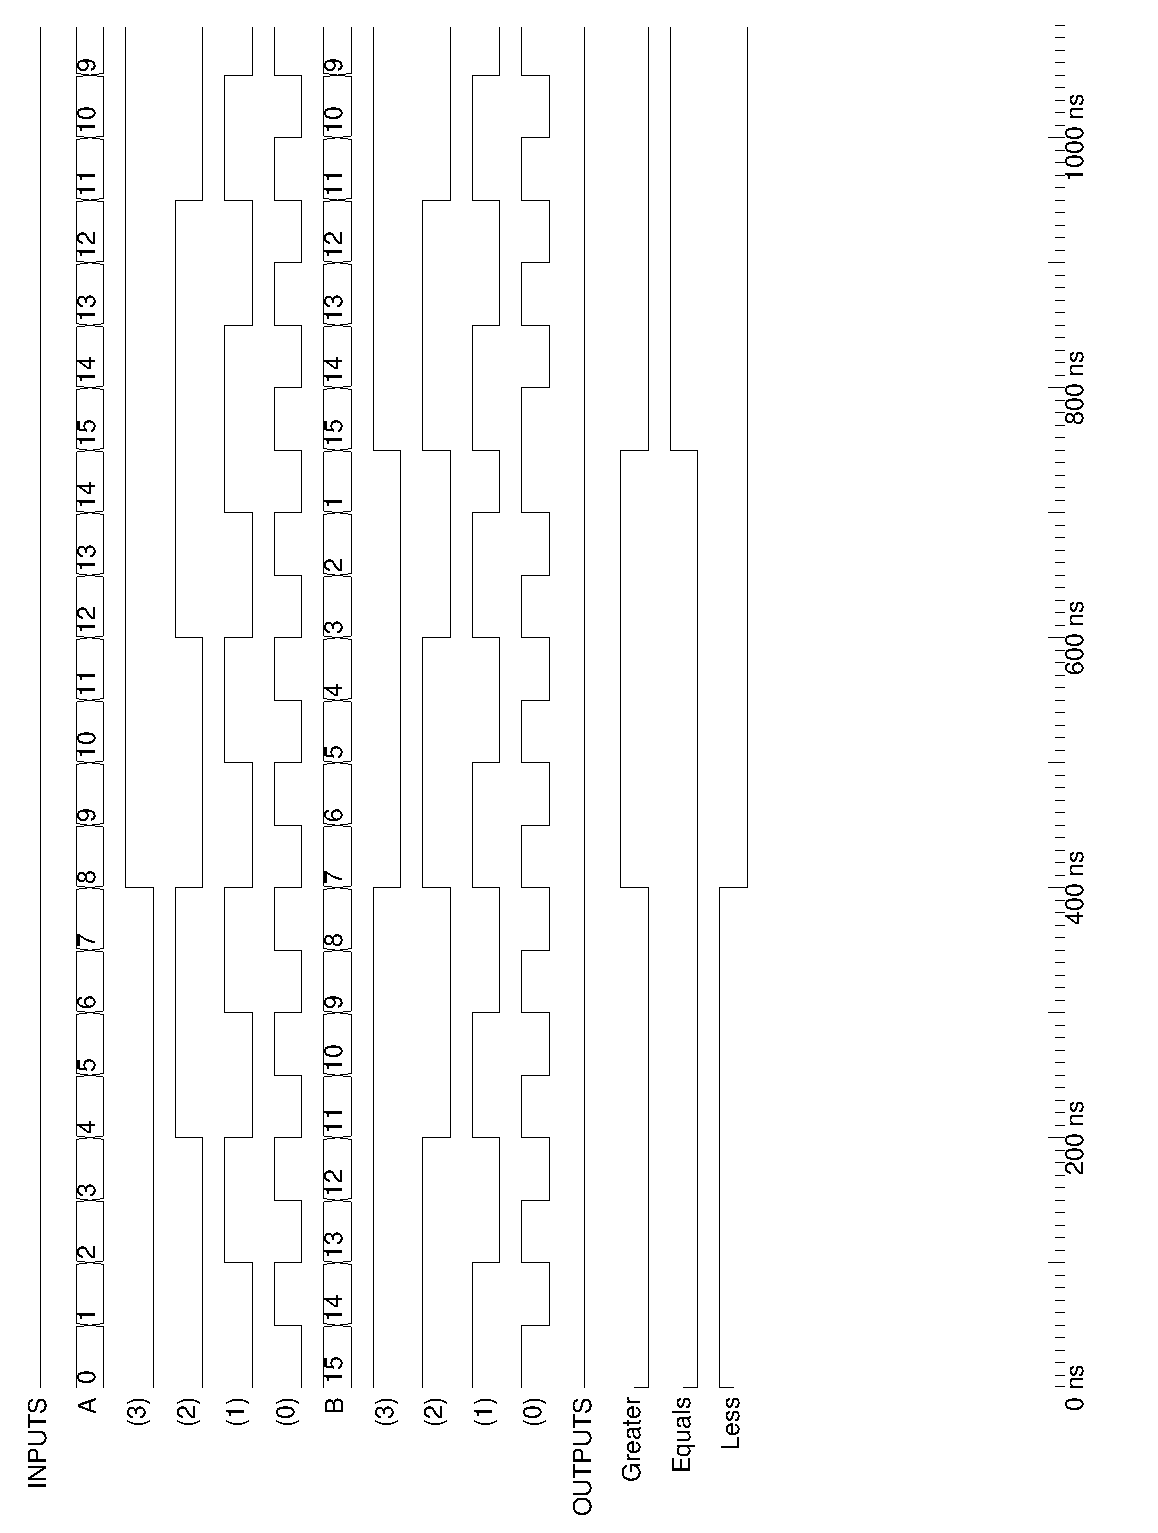
\includegraphics[scale=0.37,angle=-90]{graphs/COMP4_simulation.ps}
 \caption{\small{Simulation output with counter sequences applied
 to 4-bit inputs}}
 \end{figure}

\lstinputlisting[label=code:comp4,
caption={\emph{Behavioural Implementation of 4-bit Comparator}}]
{../code/comblogic/comparator_4bit.listing.vhd}

\pagebreak
\section{Arithmetic Logic Unit}
\subsection{Description}
\subsection{Verification}

\pagebreak
\section{Priority Encoder}
\subsection{Description}
\subsection{Verification}

\chapter{Design Units: Multifunctional Logic}

\section{ENTITY}

\subsection{Description}

%\lstinputlisting[label=code:comp4,
%caption={\emph{Behavioural Implementation of 4-bit Comparator}}]
%{../code/comblogic/comparitor_4bit.nc.vhd}

\subsection{Verification}

\end{document}
